


\begin{frame}{Sprøjte- og gødningsfrie randzoner}

\small

\begin{columns}[T]

\begin{column}{0.58\textwidth}

\textbf{Regler ved sprøjte- og gødningsfrie randzoner:}

\begin{itemize}[]
\item Følger produktionsarealer og skal være minimum 6 m brede
\item Kan ikke placeres samme sted som andre biotopplantiltag
\item Skal opretholdes i biotopplanen fra såning og frem til høst
\end{itemize}

\vspace{0.4em}

\textbf{Gavner arter:}

\footnotesize
Vilde bier, humlebier, dagsommerfugle, svirrefluer, rovbiller, græshopper, 
gul vipstjert, sanglærke, agerhøne, vibe, rødrygget tornskade, gulspurv, 
markpiber, markmus, pindsvin, lækat, flagermus, musvåge, tårnfalk

\end{column}

\begin{column}{0.40\textwidth}
\centering
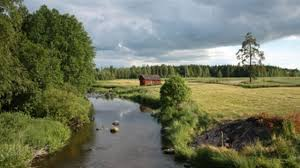
\includegraphics[width=\textwidth]{Billeder/Vildtforvaltning/biotopplantiltag/randzone.jpeg}
\end{column}

\end{columns}

\end{frame}